% Generated by Sphinx.
\def\sphinxdocclass{report}
\documentclass[letterpaper,10pt,english]{sphinxmanual}
\usepackage[utf8]{inputenc}
\DeclareUnicodeCharacter{00A0}{\nobreakspace}
\usepackage[T1]{fontenc}
\usepackage{babel}
\usepackage{times}
\usepackage[Bjarne]{fncychap}
\usepackage{longtable}
\usepackage{sphinx}
\usepackage{multirow}


\title{UChicago Physics Sample Exercises Documentation}
\date{July 22, 2014}
\release{0.1}
\author{The University of Chicago}
\newcommand{\sphinxlogo}{}
\renewcommand{\releasename}{Release}
\makeindex

\makeatletter
\def\PYG@reset{\let\PYG@it=\relax \let\PYG@bf=\relax%
    \let\PYG@ul=\relax \let\PYG@tc=\relax%
    \let\PYG@bc=\relax \let\PYG@ff=\relax}
\def\PYG@tok#1{\csname PYG@tok@#1\endcsname}
\def\PYG@toks#1+{\ifx\relax#1\empty\else%
    \PYG@tok{#1}\expandafter\PYG@toks\fi}
\def\PYG@do#1{\PYG@bc{\PYG@tc{\PYG@ul{%
    \PYG@it{\PYG@bf{\PYG@ff{#1}}}}}}}
\def\PYG#1#2{\PYG@reset\PYG@toks#1+\relax+\PYG@do{#2}}

\def\PYG@tok@gd{\def\PYG@tc##1{\textcolor[rgb]{0.63,0.00,0.00}{##1}}}
\def\PYG@tok@gu{\let\PYG@bf=\textbf\def\PYG@tc##1{\textcolor[rgb]{0.50,0.00,0.50}{##1}}}
\def\PYG@tok@gt{\def\PYG@tc##1{\textcolor[rgb]{0.00,0.25,0.82}{##1}}}
\def\PYG@tok@gs{\let\PYG@bf=\textbf}
\def\PYG@tok@gr{\def\PYG@tc##1{\textcolor[rgb]{1.00,0.00,0.00}{##1}}}
\def\PYG@tok@cm{\let\PYG@it=\textit\def\PYG@tc##1{\textcolor[rgb]{0.25,0.50,0.56}{##1}}}
\def\PYG@tok@vg{\def\PYG@tc##1{\textcolor[rgb]{0.73,0.38,0.84}{##1}}}
\def\PYG@tok@m{\def\PYG@tc##1{\textcolor[rgb]{0.13,0.50,0.31}{##1}}}
\def\PYG@tok@mh{\def\PYG@tc##1{\textcolor[rgb]{0.13,0.50,0.31}{##1}}}
\def\PYG@tok@cs{\def\PYG@tc##1{\textcolor[rgb]{0.25,0.50,0.56}{##1}}\def\PYG@bc##1{\colorbox[rgb]{1.00,0.94,0.94}{##1}}}
\def\PYG@tok@ge{\let\PYG@it=\textit}
\def\PYG@tok@vc{\def\PYG@tc##1{\textcolor[rgb]{0.73,0.38,0.84}{##1}}}
\def\PYG@tok@il{\def\PYG@tc##1{\textcolor[rgb]{0.13,0.50,0.31}{##1}}}
\def\PYG@tok@go{\def\PYG@tc##1{\textcolor[rgb]{0.19,0.19,0.19}{##1}}}
\def\PYG@tok@cp{\def\PYG@tc##1{\textcolor[rgb]{0.00,0.44,0.13}{##1}}}
\def\PYG@tok@gi{\def\PYG@tc##1{\textcolor[rgb]{0.00,0.63,0.00}{##1}}}
\def\PYG@tok@gh{\let\PYG@bf=\textbf\def\PYG@tc##1{\textcolor[rgb]{0.00,0.00,0.50}{##1}}}
\def\PYG@tok@ni{\let\PYG@bf=\textbf\def\PYG@tc##1{\textcolor[rgb]{0.84,0.33,0.22}{##1}}}
\def\PYG@tok@nl{\let\PYG@bf=\textbf\def\PYG@tc##1{\textcolor[rgb]{0.00,0.13,0.44}{##1}}}
\def\PYG@tok@nn{\let\PYG@bf=\textbf\def\PYG@tc##1{\textcolor[rgb]{0.05,0.52,0.71}{##1}}}
\def\PYG@tok@no{\def\PYG@tc##1{\textcolor[rgb]{0.38,0.68,0.84}{##1}}}
\def\PYG@tok@na{\def\PYG@tc##1{\textcolor[rgb]{0.25,0.44,0.63}{##1}}}
\def\PYG@tok@nb{\def\PYG@tc##1{\textcolor[rgb]{0.00,0.44,0.13}{##1}}}
\def\PYG@tok@nc{\let\PYG@bf=\textbf\def\PYG@tc##1{\textcolor[rgb]{0.05,0.52,0.71}{##1}}}
\def\PYG@tok@nd{\let\PYG@bf=\textbf\def\PYG@tc##1{\textcolor[rgb]{0.33,0.33,0.33}{##1}}}
\def\PYG@tok@ne{\def\PYG@tc##1{\textcolor[rgb]{0.00,0.44,0.13}{##1}}}
\def\PYG@tok@nf{\def\PYG@tc##1{\textcolor[rgb]{0.02,0.16,0.49}{##1}}}
\def\PYG@tok@si{\let\PYG@it=\textit\def\PYG@tc##1{\textcolor[rgb]{0.44,0.63,0.82}{##1}}}
\def\PYG@tok@s2{\def\PYG@tc##1{\textcolor[rgb]{0.25,0.44,0.63}{##1}}}
\def\PYG@tok@vi{\def\PYG@tc##1{\textcolor[rgb]{0.73,0.38,0.84}{##1}}}
\def\PYG@tok@nt{\let\PYG@bf=\textbf\def\PYG@tc##1{\textcolor[rgb]{0.02,0.16,0.45}{##1}}}
\def\PYG@tok@nv{\def\PYG@tc##1{\textcolor[rgb]{0.73,0.38,0.84}{##1}}}
\def\PYG@tok@s1{\def\PYG@tc##1{\textcolor[rgb]{0.25,0.44,0.63}{##1}}}
\def\PYG@tok@gp{\let\PYG@bf=\textbf\def\PYG@tc##1{\textcolor[rgb]{0.78,0.36,0.04}{##1}}}
\def\PYG@tok@sh{\def\PYG@tc##1{\textcolor[rgb]{0.25,0.44,0.63}{##1}}}
\def\PYG@tok@ow{\let\PYG@bf=\textbf\def\PYG@tc##1{\textcolor[rgb]{0.00,0.44,0.13}{##1}}}
\def\PYG@tok@sx{\def\PYG@tc##1{\textcolor[rgb]{0.78,0.36,0.04}{##1}}}
\def\PYG@tok@bp{\def\PYG@tc##1{\textcolor[rgb]{0.00,0.44,0.13}{##1}}}
\def\PYG@tok@c1{\let\PYG@it=\textit\def\PYG@tc##1{\textcolor[rgb]{0.25,0.50,0.56}{##1}}}
\def\PYG@tok@kc{\let\PYG@bf=\textbf\def\PYG@tc##1{\textcolor[rgb]{0.00,0.44,0.13}{##1}}}
\def\PYG@tok@c{\let\PYG@it=\textit\def\PYG@tc##1{\textcolor[rgb]{0.25,0.50,0.56}{##1}}}
\def\PYG@tok@mf{\def\PYG@tc##1{\textcolor[rgb]{0.13,0.50,0.31}{##1}}}
\def\PYG@tok@err{\def\PYG@bc##1{\fcolorbox[rgb]{1.00,0.00,0.00}{1,1,1}{##1}}}
\def\PYG@tok@kd{\let\PYG@bf=\textbf\def\PYG@tc##1{\textcolor[rgb]{0.00,0.44,0.13}{##1}}}
\def\PYG@tok@ss{\def\PYG@tc##1{\textcolor[rgb]{0.32,0.47,0.09}{##1}}}
\def\PYG@tok@sr{\def\PYG@tc##1{\textcolor[rgb]{0.14,0.33,0.53}{##1}}}
\def\PYG@tok@mo{\def\PYG@tc##1{\textcolor[rgb]{0.13,0.50,0.31}{##1}}}
\def\PYG@tok@mi{\def\PYG@tc##1{\textcolor[rgb]{0.13,0.50,0.31}{##1}}}
\def\PYG@tok@kn{\let\PYG@bf=\textbf\def\PYG@tc##1{\textcolor[rgb]{0.00,0.44,0.13}{##1}}}
\def\PYG@tok@o{\def\PYG@tc##1{\textcolor[rgb]{0.40,0.40,0.40}{##1}}}
\def\PYG@tok@kr{\let\PYG@bf=\textbf\def\PYG@tc##1{\textcolor[rgb]{0.00,0.44,0.13}{##1}}}
\def\PYG@tok@s{\def\PYG@tc##1{\textcolor[rgb]{0.25,0.44,0.63}{##1}}}
\def\PYG@tok@kp{\def\PYG@tc##1{\textcolor[rgb]{0.00,0.44,0.13}{##1}}}
\def\PYG@tok@w{\def\PYG@tc##1{\textcolor[rgb]{0.73,0.73,0.73}{##1}}}
\def\PYG@tok@kt{\def\PYG@tc##1{\textcolor[rgb]{0.56,0.13,0.00}{##1}}}
\def\PYG@tok@sc{\def\PYG@tc##1{\textcolor[rgb]{0.25,0.44,0.63}{##1}}}
\def\PYG@tok@sb{\def\PYG@tc##1{\textcolor[rgb]{0.25,0.44,0.63}{##1}}}
\def\PYG@tok@k{\let\PYG@bf=\textbf\def\PYG@tc##1{\textcolor[rgb]{0.00,0.44,0.13}{##1}}}
\def\PYG@tok@se{\let\PYG@bf=\textbf\def\PYG@tc##1{\textcolor[rgb]{0.25,0.44,0.63}{##1}}}
\def\PYG@tok@sd{\let\PYG@it=\textit\def\PYG@tc##1{\textcolor[rgb]{0.25,0.44,0.63}{##1}}}

\def\PYGZbs{\char`\\}
\def\PYGZus{\char`\_}
\def\PYGZob{\char`\{}
\def\PYGZcb{\char`\}}
\def\PYGZca{\char`\^}
\def\PYGZsh{\char`\#}
\def\PYGZpc{\char`\%}
\def\PYGZdl{\char`\$}
\def\PYGZti{\char`\~}
% for compatibility with earlier versions
\def\PYGZat{@}
\def\PYGZlb{[}
\def\PYGZrb{]}
\makeatother

\begin{document}

\maketitle
\tableofcontents
\phantomsection\label{index::doc}



\chapter{\texttt{Orbital} -- Launching a rocket from Mars to Earth}
\label{index:uchicago-physics-sample-exercises-s-documentation}\label{index:orbital-launching-a-rocket-from-mars-to-earth}
This problem asks the student to launch a rocket from the orbit of
Mars on a course for intercept with Earth.


\section{Build/Run}
\label{index:build-run}
\begin{Verbatim}[commandchars=\\\{\}]
\PYG{n+nv}{\PYGZdl{} }python orbital.py
\end{Verbatim}


\section{Sample Parameter file}
\label{index:sample-parameter-file}
\begin{Verbatim}[commandchars=\\\{\}]
\PYG{c}{\PYGZsh{}\PYGZsh{}\PYGZsh{}\PYGZsh{}\PYGZsh{}\PYGZsh{}\PYGZsh{}\PYGZsh{}\PYGZsh{}\PYGZsh{}\PYGZsh{}\PYGZsh{}\PYGZsh{}\PYGZsh{}\PYGZsh{}\PYGZsh{}\PYGZsh{}\PYGZsh{}\PYGZsh{}\PYGZsh{}\PYGZsh{}\PYGZsh{}\PYGZsh{}\PYGZsh{}\PYGZsh{}\PYGZsh{}\PYGZsh{}\PYGZsh{}\PYGZsh{}\PYGZsh{}\PYGZsh{}\PYGZsh{}\PYGZsh{}\PYGZsh{}\PYGZsh{}\PYGZsh{}\PYGZsh{}\PYGZsh{}\PYGZsh{}\PYGZsh{}\PYGZsh{}\PYGZsh{}\PYGZsh{}\PYGZsh{}\PYGZsh{}\PYGZsh{}\PYGZsh{}\PYGZsh{}\PYGZsh{}\PYGZsh{}\PYGZsh{}\PYGZsh{}\PYGZsh{}\PYGZsh{}\PYGZsh{}\PYGZsh{}\PYGZsh{}\PYGZsh{}\PYGZsh{}\PYGZsh{}}
\PYG{c}{\PYGZsh{} Constants and initial parameters for Martian invasion}
\PYG{c}{\PYGZsh{}\PYGZsh{}\PYGZsh{}\PYGZsh{}\PYGZsh{}\PYGZsh{}\PYGZsh{}\PYGZsh{}\PYGZsh{}\PYGZsh{}\PYGZsh{}\PYGZsh{}\PYGZsh{}\PYGZsh{}\PYGZsh{}\PYGZsh{}\PYGZsh{}\PYGZsh{}\PYGZsh{}\PYGZsh{}\PYGZsh{}\PYGZsh{}\PYGZsh{}\PYGZsh{}\PYGZsh{}\PYGZsh{}\PYGZsh{}\PYGZsh{}\PYGZsh{}\PYGZsh{}\PYGZsh{}\PYGZsh{}\PYGZsh{}\PYGZsh{}\PYGZsh{}\PYGZsh{}\PYGZsh{}\PYGZsh{}\PYGZsh{}\PYGZsh{}\PYGZsh{}\PYGZsh{}\PYGZsh{}\PYGZsh{}\PYGZsh{}\PYGZsh{}\PYGZsh{}\PYGZsh{}\PYGZsh{}\PYGZsh{}\PYGZsh{}\PYGZsh{}\PYGZsh{}\PYGZsh{}\PYGZsh{}\PYGZsh{}\PYGZsh{}\PYGZsh{}\PYGZsh{}\PYGZsh{}}

\PYG{k+kn}{import} \PYG{n+nn}{numpy} \PYG{k+kn}{as} \PYG{n+nn}{np}

\PYG{n}{MAX\PYGZus{}T}    \PYG{o}{=} \PYG{l+m+mf}{2.43e7}
\PYG{c}{\PYGZsh{} MAX\PYGZus{}T    = 3.0e7}
\PYG{n}{dt}       \PYG{o}{=} \PYG{l+m+mf}{3.6e3}    \PYG{c}{\PYGZsh{} time step of 1 hour}
\PYG{n}{MAX\PYGZus{}STEP} \PYG{o}{=} \PYG{n+nb}{int}\PYG{p}{(}\PYG{n}{MAX\PYGZus{}T}\PYG{o}{/}\PYG{n}{dt}\PYG{p}{)}
\PYG{n}{G}        \PYG{o}{=} \PYG{l+m+mf}{6.67e-11} \PYG{c}{\PYGZsh{} Gravitational constant [N m\PYGZca{}2/kg\PYGZca{}2]}

\PYG{n}{DIAM\PYGZus{}E}   \PYG{o}{=} \PYG{l+m+mf}{1.273e7}  \PYG{c}{\PYGZsh{} Diameter of the earth}
\PYG{n}{RADIUS\PYGZus{}E} \PYG{o}{=} \PYG{l+m+mf}{1.521e11} \PYG{c}{\PYGZsh{} Earth to sun           [meters]}
\PYG{n}{RADIUS\PYGZus{}M} \PYG{o}{=} \PYG{l+m+mf}{2.296e11} \PYG{c}{\PYGZsh{} mars to sun            [meters]}
\PYG{n}{RADIUS\PYGZus{}R} \PYG{o}{=} \PYG{l+m+mf}{9.281e6}  \PYG{c}{\PYGZsh{} Mars to rocket orbit   [meters]}

\PYG{n}{MASS\PYGZus{}S}   \PYG{o}{=} \PYG{l+m+mf}{1.989e30} \PYG{c}{\PYGZsh{} Mass of the Sun        [kg]}
\PYG{n}{MASS\PYGZus{}E}   \PYG{o}{=} \PYG{l+m+mf}{5.972e24} \PYG{c}{\PYGZsh{} Mass of Earth          [kg]}
\PYG{n}{MASS\PYGZus{}M}   \PYG{o}{=} \PYG{l+m+mf}{6.417e23} \PYG{c}{\PYGZsh{} Mass of Mars           [kg]}
\PYG{n}{MASS\PYGZus{}R}   \PYG{o}{=} \PYG{l+m+mf}{1.072e6}  \PYG{c}{\PYGZsh{} Mass of rocket         [kg]}

\PYG{n}{VEL\PYGZus{}E}    \PYG{o}{=} \PYG{l+m+mf}{2.98e4}   \PYG{c}{\PYGZsh{} Velocity of Earth      [m/s]}
\PYG{n}{VEL\PYGZus{}M}    \PYG{o}{=} \PYG{l+m+mf}{2.41e4}   \PYG{c}{\PYGZsh{} Velocity of Mars       [m/s]}
\PYG{n}{VEL\PYGZus{}R}    \PYG{o}{=} \PYG{l+m+mf}{2.14e3}   \PYG{c}{\PYGZsh{} Velocity of rocket     [m/s]}

\PYG{n}{R1} \PYG{o}{=} \PYG{n}{RADIUS\PYGZus{}M}\PYG{o}{-}\PYG{n}{RADIUS\PYGZus{}R}

\PYG{c}{\PYGZsh{} Hohmann boost}
\PYG{n}{V\PYGZus{}Y} \PYG{o}{=} \PYG{n}{np}\PYG{o}{.}\PYG{n}{sqrt}\PYG{p}{(}\PYG{n}{G}\PYG{o}{*}\PYG{n}{MASS\PYGZus{}S}\PYG{o}{/}\PYG{n}{R1}\PYG{p}{)}\PYG{o}{*}\PYG{p}{(}\PYG{n}{np}\PYG{o}{.}\PYG{n}{sqrt}\PYG{p}{(}\PYG{l+m+mi}{2}\PYG{o}{*}\PYG{n}{RADIUS\PYGZus{}E}\PYG{o}{/}\PYG{p}{(}\PYG{n}{RADIUS\PYGZus{}E}\PYG{o}{+}\PYG{n}{R1}\PYG{p}{)}\PYG{p}{)}\PYG{o}{-}\PYG{l+m+mi}{1}\PYG{p}{)}

\PYG{c}{\PYGZsh{} correction for numerical error of integration techinique}
\PYG{n}{V\PYGZus{}Y} \PYG{o}{*}\PYG{o}{=} \PYG{o}{.}\PYG{l+m+mi}{97}

\PYG{c}{\PYGZsh{} Secondary Hohmann boost}
\PYG{n}{V\PYGZus{}Y2} \PYG{o}{=} \PYG{n}{np}\PYG{o}{.}\PYG{n}{sqrt}\PYG{p}{(}\PYG{n}{G}\PYG{o}{*}\PYG{n}{MASS\PYGZus{}S}\PYG{o}{/}\PYG{n}{RADIUS\PYGZus{}E}\PYG{p}{)}\PYG{o}{*}\PYG{p}{(}\PYG{l+m+mi}{1}\PYG{o}{-}\PYG{n}{np}\PYG{o}{.}\PYG{n}{sqrt}\PYG{p}{(}\PYG{l+m+mi}{2}\PYG{o}{*}\PYG{n}{R1}\PYG{o}{/}\PYG{p}{(}\PYG{n}{RADIUS\PYGZus{}E}\PYG{o}{+}\PYG{n}{R1}\PYG{p}{)}\PYG{p}{)}\PYG{p}{)}
\end{Verbatim}


\section{Output}
\label{index:output}
\begin{Verbatim}[commandchars=\\\{\}]
Starting calculation.
Applying primary Hohmann boost.
Calculating trajectory.
LANDED
Plotting.
Saving plot to trajectories.png.
Plotting radii.
Saving plot to radii.png.
\end{Verbatim}

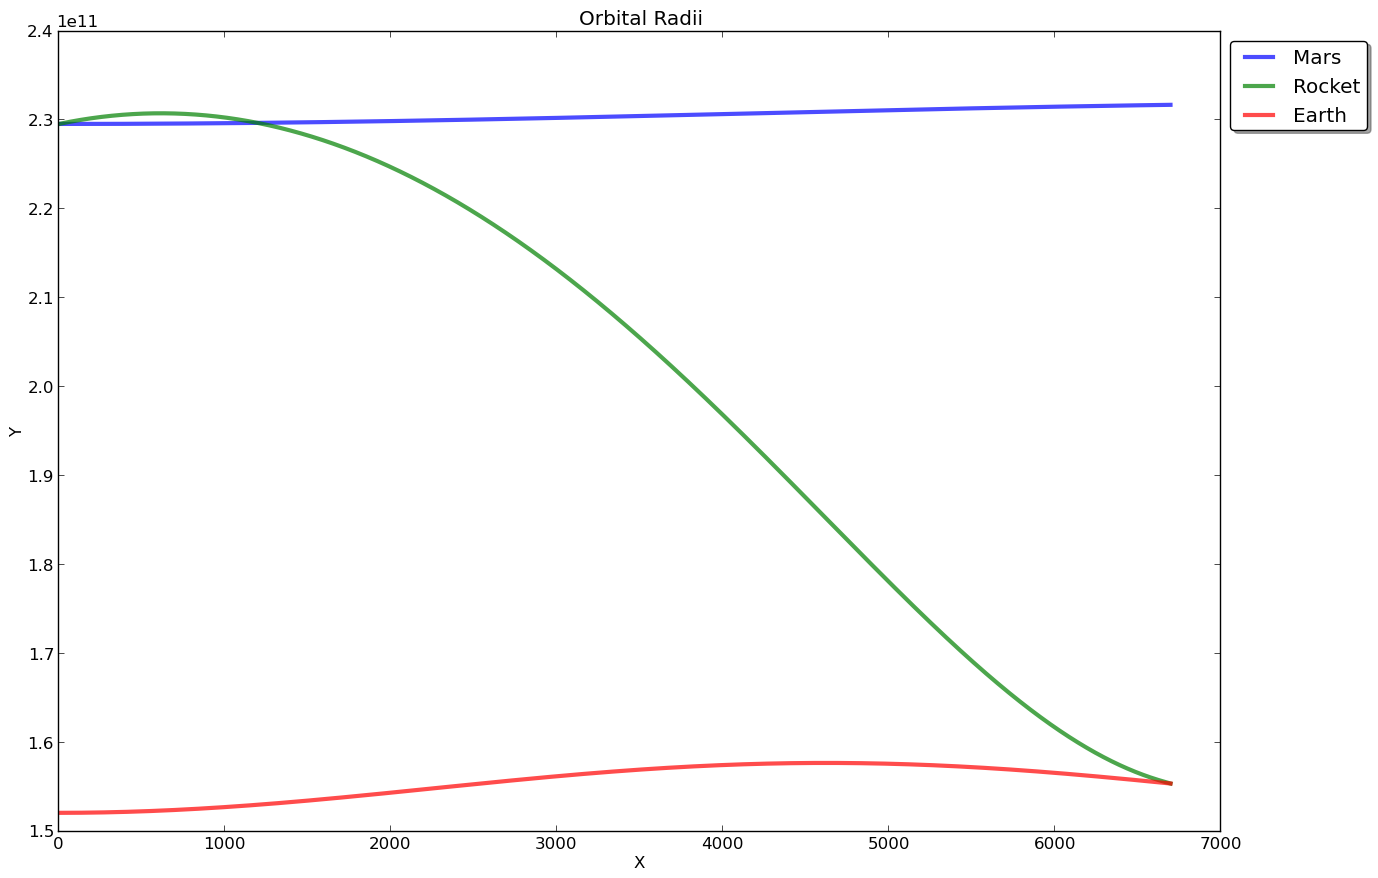
\includegraphics{radii.png}


\section{Plots}
\label{index:plots}
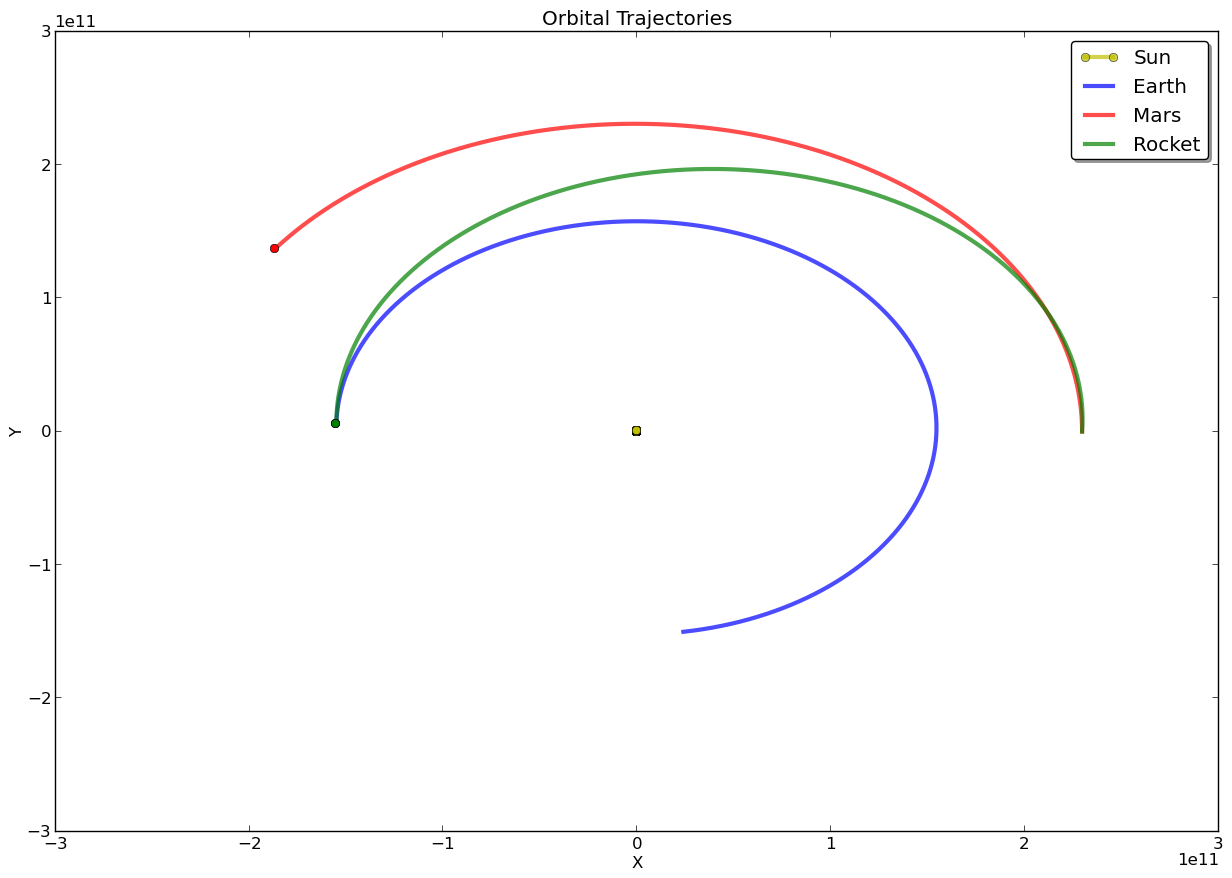
\includegraphics{trajectories.png}


\section{Methods}
\label{index:module-orbital}\label{index:methods}\index{orbital (module)}\index{calculate\_forces() (in module orbital)}

\begin{fulllineitems}
\phantomsection\label{index:orbital.calculate_forces}\pysiglinewithargsret{\code{orbital.}\bfcode{calculate\_forces}}{\emph{positions}, \emph{masses}}{}
Sum the forces on each body in the current system
\begin{quote}\begin{description}
\item[{Parameters}] \leavevmode\begin{itemize}
\item {} 
\textbf{positions} -- a two dimensional numpy array of floats: each row is a displacement vector belonging to a planetary body

\item {} 
\textbf{masses} -- a numpy array of floats: the masses of each body in kg

\end{itemize}

\item[{Returns}] \leavevmode
two dimensional numpy array of floats: an array of 2D force vectors specifying the net force on each body

\end{description}\end{quote}

\end{fulllineitems}

\index{calculate\_trajectory() (in module orbital)}

\begin{fulllineitems}
\phantomsection\label{index:orbital.calculate_trajectory}\pysiglinewithargsret{\code{orbital.}\bfcode{calculate\_trajectory}}{\emph{V\_Y}, \emph{THETA}, \emph{ADJUSTMENT}}{}
Calculates the trajectory of the rocket given the initial
Hohmann velocity boost plus gravity well adjustment
\begin{quote}\begin{description}
\item[{Parameters}] \leavevmode\begin{itemize}
\item {} 
\textbf{V\_Y} -- float: the initial Hohmann velocty boost in m/s

\item {} 
\textbf{THETA} -- the initial angular separation of Earth and Mars in radians

\item {} 
\textbf{ADJUSTMENT} -- the velocity boost adjustment needed to escape the gravity well

\end{itemize}

\end{description}\end{quote}

\end{fulllineitems}

\index{force\_gravity() (in module orbital)}

\begin{fulllineitems}
\phantomsection\label{index:orbital.force_gravity}\pysiglinewithargsret{\code{orbital.}\bfcode{force\_gravity}}{\emph{r1}, \emph{r2}, \emph{m1}, \emph{m2}}{}
Calculates the force of gravity given displacement vectors r1 \& r1
and scalar masses m1, m2
\begin{quote}\begin{description}
\item[{Parameters}] \leavevmode\begin{itemize}
\item {} 
\textbf{r1} -- numpy array of floats: the 2D cartesian location of the first body in meters

\item {} 
\textbf{r2} -- numpy array of floats: the 2D cartesian location of the second body in meters

\item {} 
\textbf{m1} -- float:  the mass of the first body in kg

\item {} 
\textbf{m2} -- float:  the mass of the first body in kg

\end{itemize}

\item[{Returns}] \leavevmode
float: the gravitational force between the two bodies in Newtons

\end{description}\end{quote}

\end{fulllineitems}

\index{plot\_orbit() (in module orbital)}

\begin{fulllineitems}
\phantomsection\label{index:orbital.plot_orbit}\pysiglinewithargsret{\code{orbital.}\bfcode{plot\_orbit}}{\emph{trajectories}}{}
plots the trajectory of each of the bodies from a birds-eye view of the Solar System. Saves output to ./trajectories.png
\begin{quote}\begin{description}
\item[{Parameters}] \leavevmode
\textbf{trajectories} -- a three dimensional numpy array: first index is time, second index is body (Sun, Earth, etc.), third index is coordinate

\item[{Returns}] \leavevmode
\code{None}

\end{description}\end{quote}

\end{fulllineitems}

\index{plot\_radii() (in module orbital)}

\begin{fulllineitems}
\phantomsection\label{index:orbital.plot_radii}\pysiglinewithargsret{\code{orbital.}\bfcode{plot\_radii}}{\emph{trajectories}}{}
plots the distance of each body from the Sun over time
\begin{quote}\begin{description}
\item[{Parameters}] \leavevmode
\textbf{trajectories} -- a three dimensional numpy array: first index is time, second index is body (Sun, Earth, etc.), third index is coordinate

\item[{Returns}] \leavevmode
\code{None}

\end{description}\end{quote}

\end{fulllineitems}

\index{update\_pos() (in module orbital)}

\begin{fulllineitems}
\phantomsection\label{index:orbital.update_pos}\pysiglinewithargsret{\code{orbital.}\bfcode{update\_pos}}{\emph{positions}, \emph{velocities}, \emph{masses}}{}
Update the positions using velocity Verlet integration
\begin{quote}\begin{description}
\item[{Parameters}] \leavevmode\begin{itemize}
\item {} 
\textbf{positions} -- a two dimensional numpy array of floats: each row is a displacement vector belonging to a planetary body

\item {} 
\textbf{positions} -- a two dimensional numpy array of floats: each row is a velocity vector belonging to a planetary body

\item {} 
\textbf{masses} -- a numpy array of floats: the masses of each body in kg

\end{itemize}

\item[{Returns}] \leavevmode
tuple length 2 of two dimensional numpy array of floats: the positions and velocities

\end{description}\end{quote}

\end{fulllineitems}



\chapter{\texttt{doublePendulum} -- Solving the Classical Double Pendulum}
\label{index:doublependulum-solving-the-classical-double-pendulum}
Solve the classical double pendulum problem.  This problem is
appropriate for an intermediate mechanics course teach Lagrangian and
Hamiltonian Dynamics.


\section{Build/Run}
\label{index:id1}
\begin{Verbatim}[commandchars=\\\{\}]
\PYG{n+nv}{\PYGZdl{} }python doublePendulum.py
\end{Verbatim}


\section{Sample Parameter file}
\label{index:id2}
\begin{Verbatim}[commandchars=\\\{\}]
\PYG{c}{\PYGZsh{}\PYGZsh{}\PYGZsh{}\PYGZsh{}\PYGZsh{}\PYGZsh{}\PYGZsh{}\PYGZsh{}\PYGZsh{}\PYGZsh{}\PYGZsh{}\PYGZsh{}\PYGZsh{}\PYGZsh{}\PYGZsh{}\PYGZsh{}\PYGZsh{}\PYGZsh{}\PYGZsh{}\PYGZsh{}\PYGZsh{}\PYGZsh{}\PYGZsh{}\PYGZsh{}\PYGZsh{}\PYGZsh{}\PYGZsh{}\PYGZsh{}\PYGZsh{}\PYGZsh{}\PYGZsh{}\PYGZsh{}\PYGZsh{}\PYGZsh{}\PYGZsh{}\PYGZsh{}\PYGZsh{}\PYGZsh{}\PYGZsh{}\PYGZsh{}\PYGZsh{}\PYGZsh{}\PYGZsh{}\PYGZsh{}\PYGZsh{}\PYGZsh{}\PYGZsh{}\PYGZsh{}\PYGZsh{}\PYGZsh{}\PYGZsh{}\PYGZsh{}\PYGZsh{}\PYGZsh{}\PYGZsh{}\PYGZsh{}\PYGZsh{}\PYGZsh{}\PYGZsh{}\PYGZsh{}}
\PYG{c}{\PYGZsh{} Double Pendulum Parameter file}
\PYG{c}{\PYGZsh{}\PYGZsh{}\PYGZsh{}\PYGZsh{}\PYGZsh{}\PYGZsh{}\PYGZsh{}\PYGZsh{}\PYGZsh{}\PYGZsh{}\PYGZsh{}\PYGZsh{}\PYGZsh{}\PYGZsh{}\PYGZsh{}\PYGZsh{}\PYGZsh{}\PYGZsh{}\PYGZsh{}\PYGZsh{}\PYGZsh{}\PYGZsh{}\PYGZsh{}\PYGZsh{}\PYGZsh{}\PYGZsh{}\PYGZsh{}\PYGZsh{}\PYGZsh{}\PYGZsh{}\PYGZsh{}\PYGZsh{}\PYGZsh{}\PYGZsh{}\PYGZsh{}\PYGZsh{}\PYGZsh{}\PYGZsh{}\PYGZsh{}\PYGZsh{}\PYGZsh{}\PYGZsh{}\PYGZsh{}\PYGZsh{}\PYGZsh{}\PYGZsh{}\PYGZsh{}\PYGZsh{}\PYGZsh{}\PYGZsh{}\PYGZsh{}\PYGZsh{}\PYGZsh{}\PYGZsh{}\PYGZsh{}\PYGZsh{}\PYGZsh{}\PYGZsh{}\PYGZsh{}\PYGZsh{}}

\PYG{k+kn}{import} \PYG{n+nn}{numpy} \PYG{k+kn}{as} \PYG{n+nn}{np}

\PYG{n}{g} \PYG{o}{=} \PYG{l+m+mf}{9.8}                  \PYG{c}{\PYGZsh{} m/s}

\PYG{n}{l1}       \PYG{o}{=} \PYG{l+m+mf}{1.2}           \PYG{c}{\PYGZsh{} m}
\PYG{n}{l2}       \PYG{o}{=} \PYG{o}{.}\PYG{l+m+mi}{7}            \PYG{c}{\PYGZsh{}m}

\PYG{n}{theta1\PYGZus{}0} \PYG{o}{=} \PYG{n}{np}\PYG{o}{.}\PYG{n}{pi}\PYG{o}{/}\PYG{l+m+mi}{4}
\PYG{n}{theta2\PYGZus{}0} \PYG{o}{=} \PYG{n}{np}\PYG{o}{.}\PYG{n}{pi}

\PYG{n}{m1}       \PYG{o}{=} \PYG{o}{.}\PYG{l+m+mi}{10}           \PYG{c}{\PYGZsh{} kg}
\PYG{n}{m2}       \PYG{o}{=} \PYG{o}{.}\PYG{l+m+mo}{05}           \PYG{c}{\PYGZsh{} kg}

\PYG{n}{dt}       \PYG{o}{=} \PYG{l+m+mf}{1e-3}
\PYG{n}{max\PYGZus{}t}    \PYG{o}{=} \PYG{l+m+mf}{5.0}

\PYG{n}{nsteps}   \PYG{o}{=} \PYG{n+nb}{int}\PYG{p}{(}\PYG{n}{max\PYGZus{}t}\PYG{o}{/}\PYG{n}{dt}\PYG{p}{)} \PYG{c}{\PYGZsh{} number of steps}

\PYG{k}{print} \PYG{l+s}{"}\PYG{l+s}{nsteps:}\PYG{l+s}{"}\PYG{p}{,} \PYG{n}{nsteps}
\end{Verbatim}


\section{Output}
\label{index:id3}
\begin{Verbatim}[commandchars=\\\{\}]
nsteps: 5000
Starting calculation.
Plotting.
Saving plot to pendulum.png.
nsteps: 5000
Starting calculation.
Plotting.
Saving plot to pendulum.png.
\end{Verbatim}


\section{Plots}
\label{index:id4}
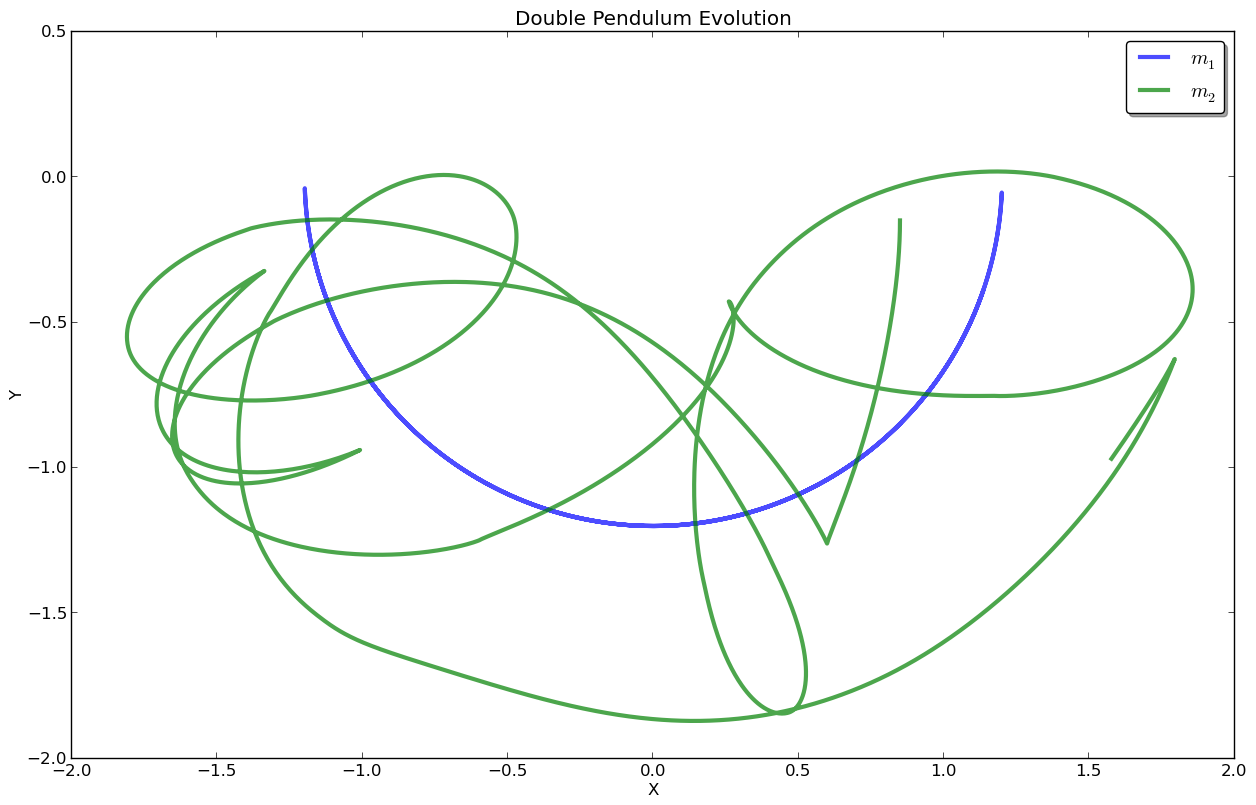
\includegraphics{pendulum.png}


\section{Methods}
\label{index:id5}\phantomsection\label{index:module-doublePendulum}\index{doublePendulum (module)}\index{C1() (in module doublePendulum)}

\begin{fulllineitems}
\phantomsection\label{index:doublePendulum.C1}\pysiglinewithargsret{\code{doublePendulum.}\bfcode{C1}}{\emph{theta1}, \emph{theta2}, \emph{p1}, \emph{p2}}{}
helper function to calculate a constant \code{C\_1}
\begin{quote}\begin{description}
\item[{Parameters}] \leavevmode\begin{itemize}
\item {} 
\textbf{theta1} -- float

\item {} 
\textbf{theta2} -- float

\item {} 
\textbf{p1} -- float

\item {} 
\textbf{p2} -- float

\end{itemize}

\item[{Returns}] \leavevmode
float, constant used in calculating Hamilton's equation

\end{description}\end{quote}

\end{fulllineitems}

\index{C2() (in module doublePendulum)}

\begin{fulllineitems}
\phantomsection\label{index:doublePendulum.C2}\pysiglinewithargsret{\code{doublePendulum.}\bfcode{C2}}{\emph{theta1}, \emph{theta2}, \emph{p1}, \emph{p2}}{}
helper function to calculate a constant \code{C\_2}
\begin{quote}\begin{description}
\item[{Parameters}] \leavevmode\begin{itemize}
\item {} 
\textbf{theta1} -- float

\item {} 
\textbf{theta2} -- float

\item {} 
\textbf{p1} -- float

\item {} 
\textbf{p2} -- float

\end{itemize}

\item[{Returns}] \leavevmode
float, constant used in calculating Hamilton's equation

\end{description}\end{quote}

\end{fulllineitems}

\index{calculate\_paths() (in module doublePendulum)}

\begin{fulllineitems}
\phantomsection\label{index:doublePendulum.calculate_paths}\pysiglinewithargsret{\code{doublePendulum.}\bfcode{calculate\_paths}}{\emph{method='euler'}}{}
use a default or specified method of integration to solve the
pendulum's motion
\begin{quote}\begin{description}
\item[{Parameters}] \leavevmode
\textbf{method} -- optional, string.  specify the integration method to use

\end{description}\end{quote}

\end{fulllineitems}

\index{deriv() (in module doublePendulum)}

\begin{fulllineitems}
\phantomsection\label{index:doublePendulum.deriv}\pysiglinewithargsret{\code{doublePendulum.}\bfcode{deriv}}{\emph{t}, \emph{y}}{}
calculated the derivative of \code{theta1, theta2, p1, p2}
\begin{quote}\begin{description}
\item[{Parameters}] \leavevmode\begin{itemize}
\item {} 
\textbf{theta1} -- float

\item {} 
\textbf{theta2} -- float

\item {} 
\textbf{p1} -- float

\item {} 
\textbf{p2} -- float

\end{itemize}

\item[{Returns}] \leavevmode
numpy array, time derivative of parameters

\end{description}\end{quote}

\end{fulllineitems}

\index{dp1() (in module doublePendulum)}

\begin{fulllineitems}
\phantomsection\label{index:doublePendulum.dp1}\pysiglinewithargsret{\code{doublePendulum.}\bfcode{dp1}}{\emph{theta1}, \emph{theta2}, \emph{p1}, \emph{p2}, \emph{c1}, \emph{c2}}{}
the time derivative of \code{p1}
\begin{quote}\begin{description}
\item[{Parameters}] \leavevmode\begin{itemize}
\item {} 
\textbf{theta1} -- float

\item {} 
\textbf{theta2} -- float

\item {} 
\textbf{p1} -- float

\item {} 
\textbf{p2} -- float

\end{itemize}

\item[{Returns}] \leavevmode
float, the time derivative of p1

\end{description}\end{quote}

\end{fulllineitems}

\index{dp2() (in module doublePendulum)}

\begin{fulllineitems}
\phantomsection\label{index:doublePendulum.dp2}\pysiglinewithargsret{\code{doublePendulum.}\bfcode{dp2}}{\emph{theta1}, \emph{theta2}, \emph{p1}, \emph{p2}, \emph{c1}, \emph{c2}}{}
the time derivative of \code{p2}
\begin{quote}\begin{description}
\item[{Parameters}] \leavevmode\begin{itemize}
\item {} 
\textbf{theta1} -- float

\item {} 
\textbf{theta2} -- float

\item {} 
\textbf{p1} -- float

\item {} 
\textbf{p2} -- float

\end{itemize}

\item[{Returns}] \leavevmode
float, the time derivative of p2

\end{description}\end{quote}

\end{fulllineitems}

\index{dtheta1() (in module doublePendulum)}

\begin{fulllineitems}
\phantomsection\label{index:doublePendulum.dtheta1}\pysiglinewithargsret{\code{doublePendulum.}\bfcode{dtheta1}}{\emph{theta1}, \emph{theta2}, \emph{p1}, \emph{p2}}{}
the time derivative of \code{theta1}
\begin{quote}\begin{description}
\item[{Parameters}] \leavevmode\begin{itemize}
\item {} 
\textbf{theta1} -- float

\item {} 
\textbf{theta2} -- float

\item {} 
\textbf{p1} -- float

\item {} 
\textbf{p2} -- float

\end{itemize}

\item[{Returns}] \leavevmode
float, the time derivative of theta1

\end{description}\end{quote}

\end{fulllineitems}

\index{dtheta2() (in module doublePendulum)}

\begin{fulllineitems}
\phantomsection\label{index:doublePendulum.dtheta2}\pysiglinewithargsret{\code{doublePendulum.}\bfcode{dtheta2}}{\emph{theta1}, \emph{theta2}, \emph{p1}, \emph{p2}}{}
the time derivative of \code{theta2}
\begin{quote}\begin{description}
\item[{Parameters}] \leavevmode\begin{itemize}
\item {} 
\textbf{theta1} -- float

\item {} 
\textbf{theta2} -- float

\item {} 
\textbf{p1} -- float

\item {} 
\textbf{p2} -- float

\end{itemize}

\item[{Returns}] \leavevmode
float, the time derivative of theta2

\end{description}\end{quote}

\end{fulllineitems}

\index{euler() (in module doublePendulum)}

\begin{fulllineitems}
\phantomsection\label{index:doublePendulum.euler}\pysiglinewithargsret{\code{doublePendulum.}\bfcode{euler}}{\emph{theta1}, \emph{theta2}, \emph{p1}, \emph{p2}}{}
use a naive euler integration schemed to make a single step in
the pendulum's motion
\begin{quote}\begin{description}
\item[{Parameters}] \leavevmode\begin{itemize}
\item {} 
\textbf{theta1} -- float

\item {} 
\textbf{theta2} -- float

\item {} 
\textbf{p1} -- float

\item {} 
\textbf{p2} -- float

\end{itemize}

\item[{Returns}] \leavevmode
tuple of updated parameters

\end{description}\end{quote}

\end{fulllineitems}

\index{velocity\_verlet() (in module doublePendulum)}

\begin{fulllineitems}
\phantomsection\label{index:doublePendulum.velocity_verlet}\pysiglinewithargsret{\code{doublePendulum.}\bfcode{velocity\_verlet}}{\emph{theta1}, \emph{theta2}, \emph{p1}, \emph{p2}}{}
\textbf{TODO} use a velocity verlet integration schemed to make a single step in
the pendulum's motion
\begin{quote}\begin{description}
\item[{Parameters}] \leavevmode\begin{itemize}
\item {} 
\textbf{theta1} -- float

\item {} 
\textbf{theta2} -- float

\item {} 
\textbf{p1} -- float

\item {} 
\textbf{p2} -- float

\end{itemize}

\item[{Returns}] \leavevmode
tuple of parameters

\end{description}\end{quote}

\end{fulllineitems}

\phantomsection\label{index:module-plotting}\index{plotting (module)}\index{animate() (in module plotting)}

\begin{fulllineitems}
\phantomsection\label{index:plotting.animate}\pysiglinewithargsret{\code{plotting.}\bfcode{animate}}{\emph{i}}{}
Helper function for {\hyperref[index:plotting.animate_paths]{\code{animate\_paths()}}}. Adds the objects and
paths to the plot for each frame
\begin{quote}\begin{description}
\item[{Parameters}] \leavevmode
\textbf{i} -- the frame number

\item[{Returns}] \leavevmode
\code{None}

\end{description}\end{quote}

\end{fulllineitems}

\index{animate\_paths() (in module plotting)}

\begin{fulllineitems}
\phantomsection\label{index:plotting.animate_paths}\pysiglinewithargsret{\code{plotting.}\bfcode{animate\_paths}}{\emph{paths}, \emph{dt}}{}
Animate the images by compiling .png outputs into a .mp4 video. \textbf{REQUIRES: ffmpeg}
\begin{quote}\begin{description}
\item[{Parameters}] \leavevmode\begin{itemize}
\item {} 
\textbf{paths} -- a three dimensional numpy array: The first index is over time, the second specifies which mass, the third specifies the cartesian displacement

\item {} 
\textbf{dt} -- the timestep in seconds

\end{itemize}

\item[{Returns}] \leavevmode
\code{None}

\end{description}\end{quote}

\end{fulllineitems}

\index{plot\_paths() (in module plotting)}

\begin{fulllineitems}
\phantomsection\label{index:plotting.plot_paths}\pysiglinewithargsret{\code{plotting.}\bfcode{plot\_paths}}{\emph{paths}}{}
Plot the paths to a png image \code{./pendulum.png}.
\begin{quote}\begin{description}
\item[{Parameters}] \leavevmode
\textbf{paths} -- a three dimensional numpy array: The first index is over time, the second specifies which mass, the third specifies the cartesian displacement

\item[{Returns}] \leavevmode
\code{None}

\end{description}\end{quote}

\end{fulllineitems}



\chapter{\texttt{electronTrajectory} -- Comparing Trajectory of Charged Particles in a Magnetic Field}
\label{index:electrontrajectory-comparing-trajectory-of-charged-particles-in-a-magnetic-field}
Calculate the trajectory of charged particles with different masses in
an external magnetic field.


\section{Build/Run}
\label{index:id6}
\begin{Verbatim}[commandchars=\\\{\}]
\PYG{n+nv}{\PYGZdl{} }python electronTrajectory.py
\end{Verbatim}


\section{Output}
\label{index:id7}
\begin{Verbatim}[commandchars=\\\{\}]
Starting calculation.
Calculating trajectory: 9.11e-31 kg
Calculating trajectory: 1.82e-30 kg
Calculating trajectory: 2.73e-30 kg
Calculating trajectory: 3.64e-30 kg
Calculating trajectory: 4.55e-30 kg
Calculating trajectory: 5.47e-30 kg
Plotting.
Saving plot to trajectory.png.
\end{Verbatim}


\section{Plots}
\label{index:id8}
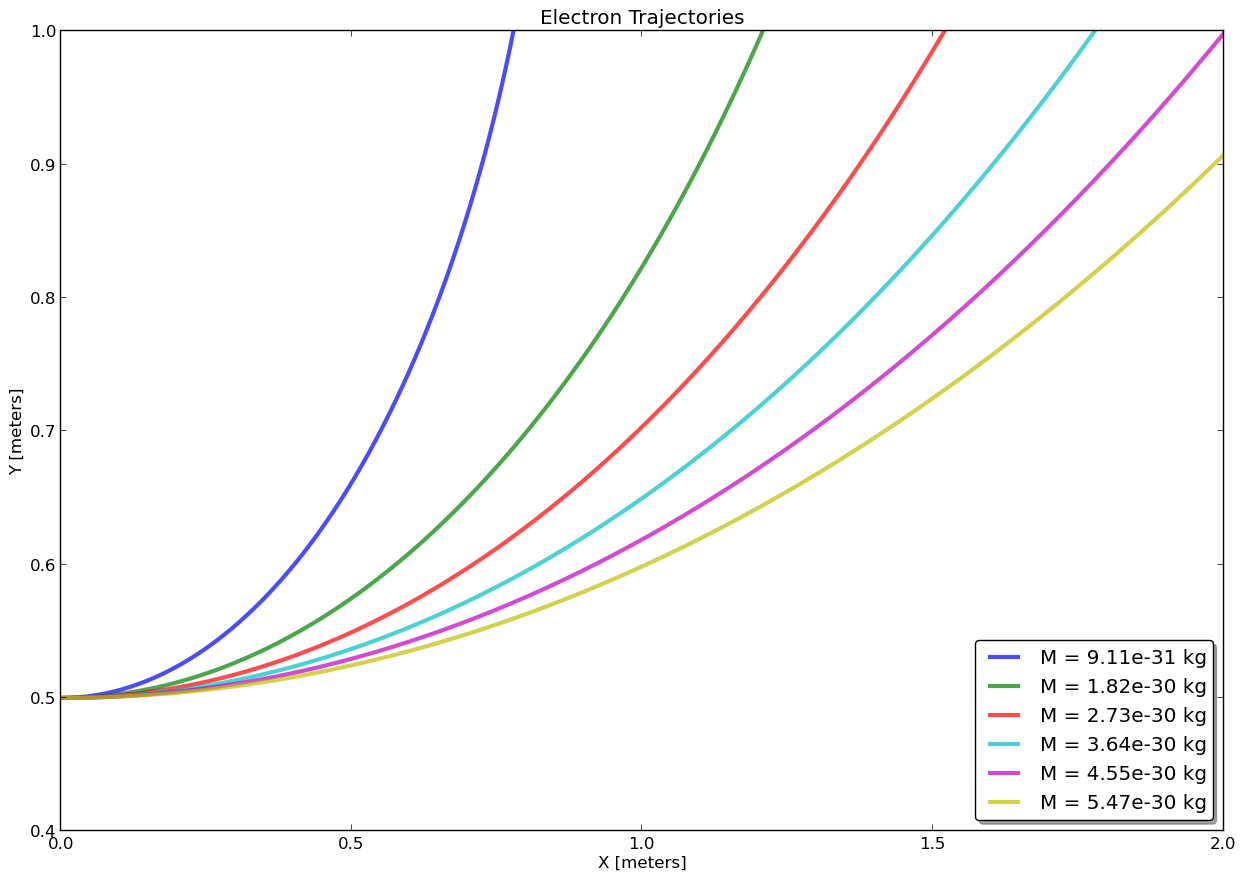
\includegraphics{trajectory.png}


\section{Methods}
\label{index:id9}\phantomsection\label{index:module-electronTrajectory}\index{electronTrajectory (module)}\index{calculate\_trajectory() (in module electronTrajectory)}

\begin{fulllineitems}
\phantomsection\label{index:electronTrajectory.calculate_trajectory}\pysiglinewithargsret{\code{electronTrajectory.}\bfcode{calculate\_trajectory}}{\emph{position}, \emph{velocity}, \emph{mass}, \emph{B}}{}
Calculates the trajectory of the particle
\begin{quote}\begin{description}
\item[{Parameters}] \leavevmode\begin{itemize}
\item {} 
\textbf{position} -- 3D vector (r\_x,r\_y,r\_z) in meters

\item {} 
\textbf{velocity} -- 3D vector (v\_x,v\_y,v\_z) in m/s

\item {} 
\textbf{mass} -- scalar float in kg

\item {} 
\textbf{B} -- magnetic field strength, scalar float in Tesla

\end{itemize}

\item[{Returns}] \leavevmode
a numpy array of 3D vectors (np.arrays)

\end{description}\end{quote}

\end{fulllineitems}

\index{main() (in module electronTrajectory)}

\begin{fulllineitems}
\phantomsection\label{index:electronTrajectory.main}\pysiglinewithargsret{\code{electronTrajectory.}\bfcode{main}}{}{}
Loops over particles with integer multiples of the mass of the
electron and shoots them through the magnetic field

\end{fulllineitems}

\index{plot\_trajectory() (in module electronTrajectory)}

\begin{fulllineitems}
\phantomsection\label{index:electronTrajectory.plot_trajectory}\pysiglinewithargsret{\code{electronTrajectory.}\bfcode{plot\_trajectory}}{\emph{trajectories}, \emph{masses}}{}
Creates a matplotlib plot and plots a list of trajectories labeled
by a list of masses.


\strong{See Also:}


called by {\hyperref[index:electronTrajectory.main]{\code{main()}}}


\begin{quote}\begin{description}
\item[{Parameters}] \leavevmode
\textbf{trajectories} -- an array of trajectories

\end{description}\end{quote}

:param masses:: a list of masses
:returns: \code{None}

\end{fulllineitems}

\index{update\_pos() (in module electronTrajectory)}

\begin{fulllineitems}
\phantomsection\label{index:electronTrajectory.update_pos}\pysiglinewithargsret{\code{electronTrajectory.}\bfcode{update\_pos}}{\emph{position}, \emph{velocity}, \emph{mass}, \emph{B}}{}
calculates the magnetic force on the particle and moves it
accordingly
\begin{quote}\begin{description}
\item[{Parameters}] \leavevmode\begin{itemize}
\item {} 
\textbf{position} -- 3D numpy array (r\_x,r\_y,r\_z) in meters

\item {} 
\textbf{velocity} -- 3D numpy array (v\_x,v\_y,v\_z) in m/s

\item {} 
\textbf{mass} -- scalar float in kg

\item {} 
\textbf{B} -- magnetic field strength, scalar float in Tesla

\end{itemize}

\item[{Returns}] \leavevmode
the updated position and velocity (3D vectors)

\end{description}\end{quote}

\end{fulllineitems}



\renewcommand{\indexname}{Python Module Index}
\begin{theindex}
\def\bigletter#1{{\Large\sffamily#1}\nopagebreak\vspace{1mm}}
\bigletter{d}
\item {\texttt{doublePendulum}}, \pageref{index:module-doublePendulum}
\indexspace
\bigletter{e}
\item {\texttt{electronTrajectory}}, \pageref{index:module-electronTrajectory}
\indexspace
\bigletter{o}
\item {\texttt{orbital}}, \pageref{index:module-orbital}
\indexspace
\bigletter{p}
\item {\texttt{plotting}}, \pageref{index:module-plotting}
\end{theindex}

\renewcommand{\indexname}{Index}
\printindex
\end{document}
